\subsection{Harder Problems Often Lead to Better Performance}
\label{subsubsec:harder_better}

\begin{figure*}[htbp]
    \centering
    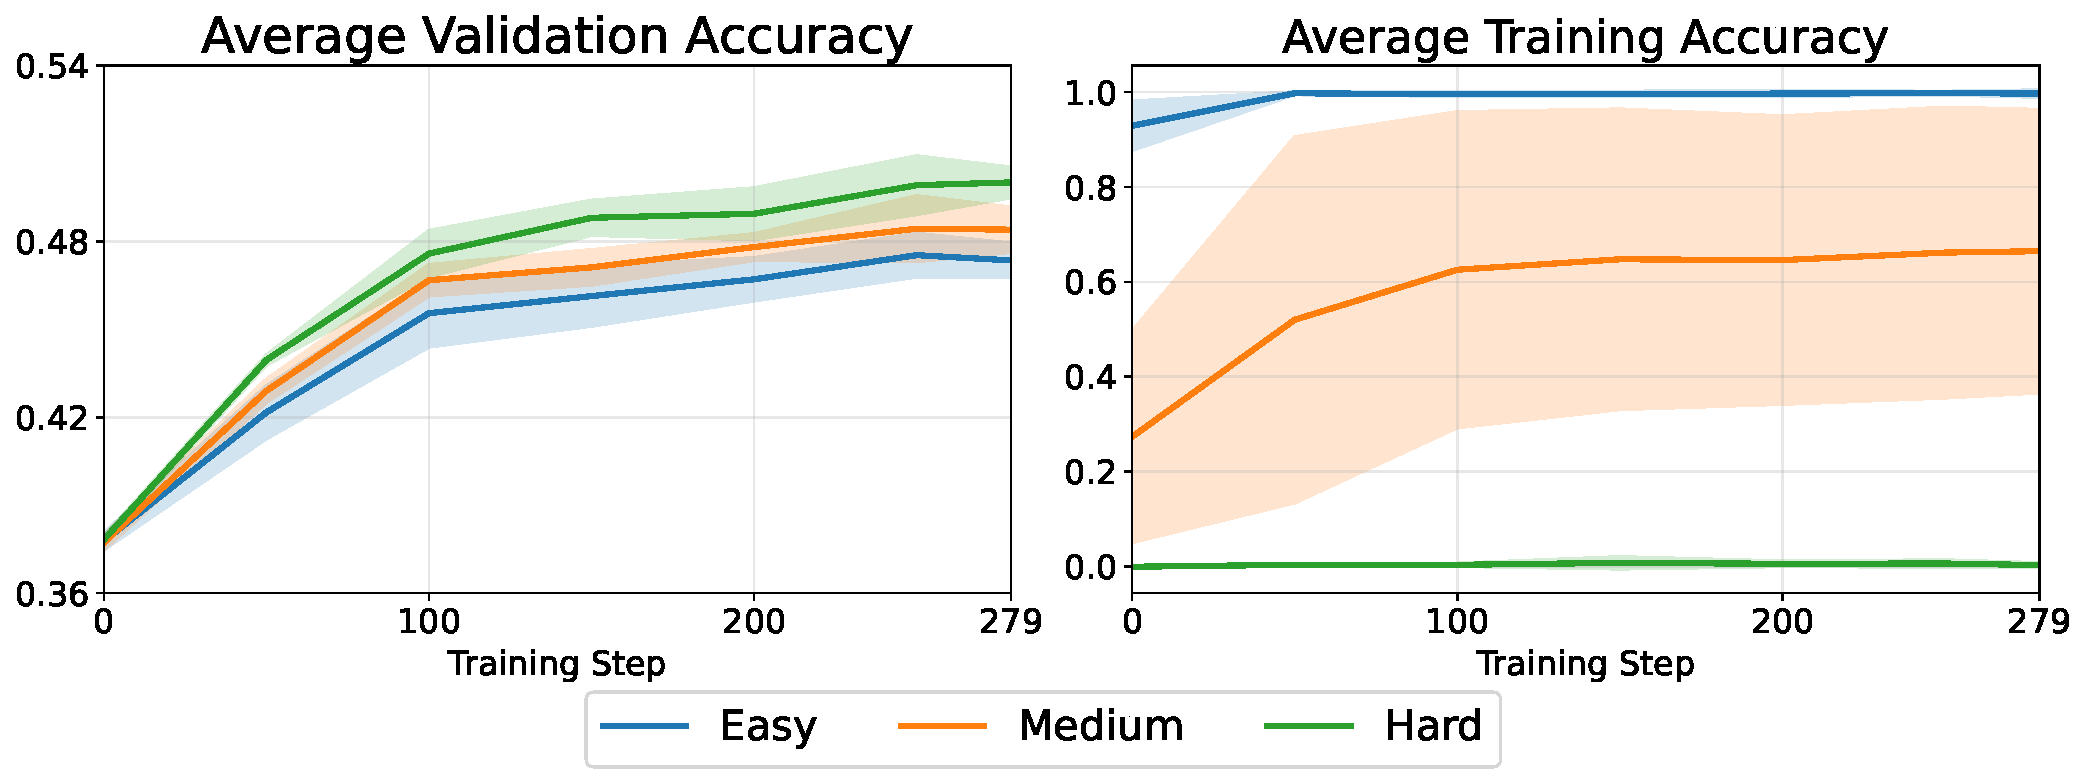
\includegraphics[width=\textwidth]{./images/difficulty.pdf}
    \caption{\textbf{Learning Trajectories across Difficulty Levels.} Left: Average Validation Accuracy over training steps. Right: Average Training Accuracy on the selected training example over training steps. Solid lines indicate the mean and shaded areas represent the standard deviation across the examples in each category.}
    \label{fig:difficulty_curves}
\end{figure*}

We further investigate whether different data behave differently in 1-shot OPD. For each category, we record both the average training accuracy and validation accuracy every 50 training steps, and present these trajectories in Figure \ref{fig:difficulty_curves}. Surprisingly, we find that harder training examples often yield better performance. Moreover, we observe that for easy and hard problems, even after their training accuracies saturate at 100\% (for easy tasks) or remain flat at 0\% (for hard tasks), their validation accuracies continuously improve. This behavior contrasts sharply with RL (e.g., GRPO-style algorithms) where training on extreme easy and hard samples is highly ineffective because the computed advantage or gradient updates tend to be zero.


\subsection{Deeper Analysis}
\label{subsec:entropy_vs_cot}
We next explore what underlying properties drive the efficacy of difficult prompts, examining potential factors such as the higher token entropy and the longer CoT reasoning sequences they naturally generate. 

\begin{figure}[t]
    \centering
    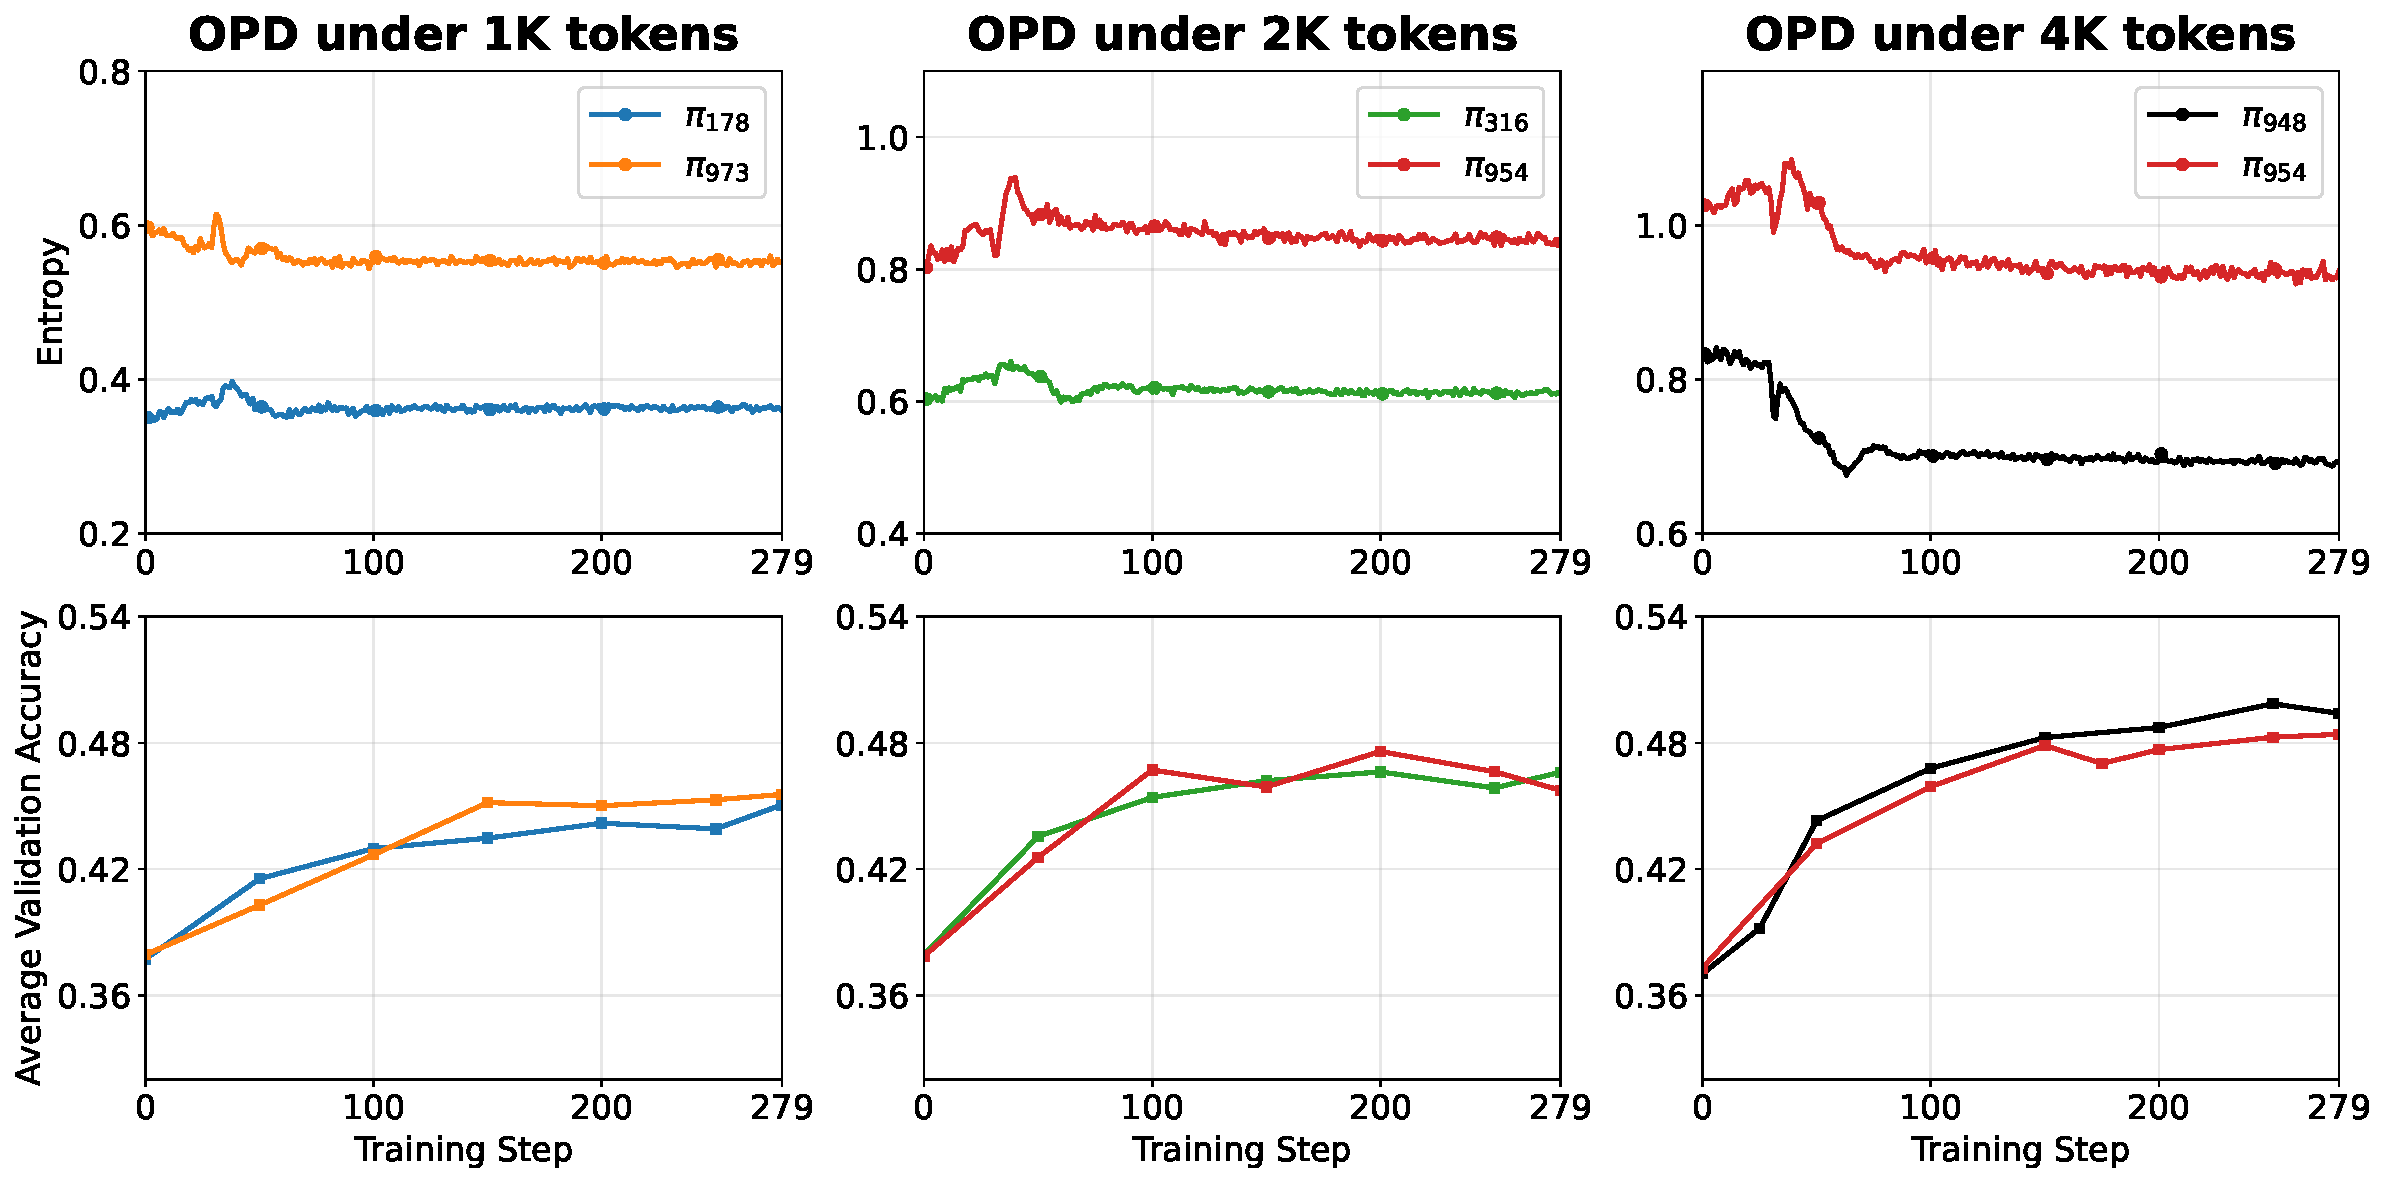
\includegraphics[width=\linewidth]{./images/short.pdf}
    \caption{\textbf{Training Dynamics in Length-Constrained Setting}  Training dynamics are presented for problem pairs grouped by difficulty: Easy vs. Hard (1K token limit, left), Medium vs. Hard (2K token limit, middle), and Hard vs. Hard (4K token limit, right). The top plots monitor token entropy, while the bottom plots track validation accuracy.}
    \label{fig:cot_truncation_gap}
\end{figure}

\textbf{Setup.} To isolate the role of token entropy from length related factors, we set up a length-controlled experiment. By adjusting the maximum rollout length, we expect that almost all rollouts generated for some examples will exceed this limit and get cut off. Consequently, training the 1-shot OPD uses almost the same number of tokens for those examples because the length of every response is forced to be the maximum rollout length. Specifically, we conduct three sets of experiments. In each set, we select two problems with different difficulty or entropy, and set an appropriate maximum rollout length such that empirically over 99.5\% of the rollouts for both problems exceed this threshold. The three problem pairs are: 1) Easy problem $\pi_{178}$ and Hard problem $\pi_{973}$ limited to $1024$ tokens, 2) Medium problem $\pi_{316}$ and Hard problem $\pi_{954}$ limited to $2048$ tokens, and 3) two Hard problems with highly different token entropy, $\pi_{948}$ and $\pi_{954}$ limited to $4096$ tokens.


\textbf{Higher Token Entropy Alone Does Not Improve OPD} As illustrated in Figure~\ref{fig:cot_truncation_gap}, under length-controlled settings, we observe no  significant difference in validation performance between the compared pairs, despite their highly divergent token entropy. Specifically, once rollout lengths are restricted to match, the performance gap between the pairs collapses to $0.5\%$ (for $\{\pi_{973}\}$ vs. $\{\pi_{178}\}$) and $-0.9\%$ (for $\{\pi_{954}\}$ vs. $\{\pi_{316}\}$). However, in the default setting (7,168 maximum rollout length) where the student model can leverage the longer CoT sequences generated by harder examples, the harder problems demonstrate a notable advantage, outperforming $\{\pi_{178}\}$ and $\{\pi_{316}\}$ by $3.9\%$ and $2.4\%$ in validation accuracy, respectively. This collapse under length limits indicates that higher token entropy alone does not translate to better distillation performance. Additionally, we perform an auxiliary experiment where we sample responses for the Easy problem $\pi_{178}$ under higher temperatures to artificially increase token entropy. As shown in Figure \ref{fig:temperature}, the resulting model shows no accuracy gains, indicating that the performance improvement of difficult tasks is not driven by their higher token entropy.



\begin{wrapfigure}{r}{0.4\linewidth} % r 表示图片在右侧，占用 50% 宽度
    \vspace{-1em}
    \centering
    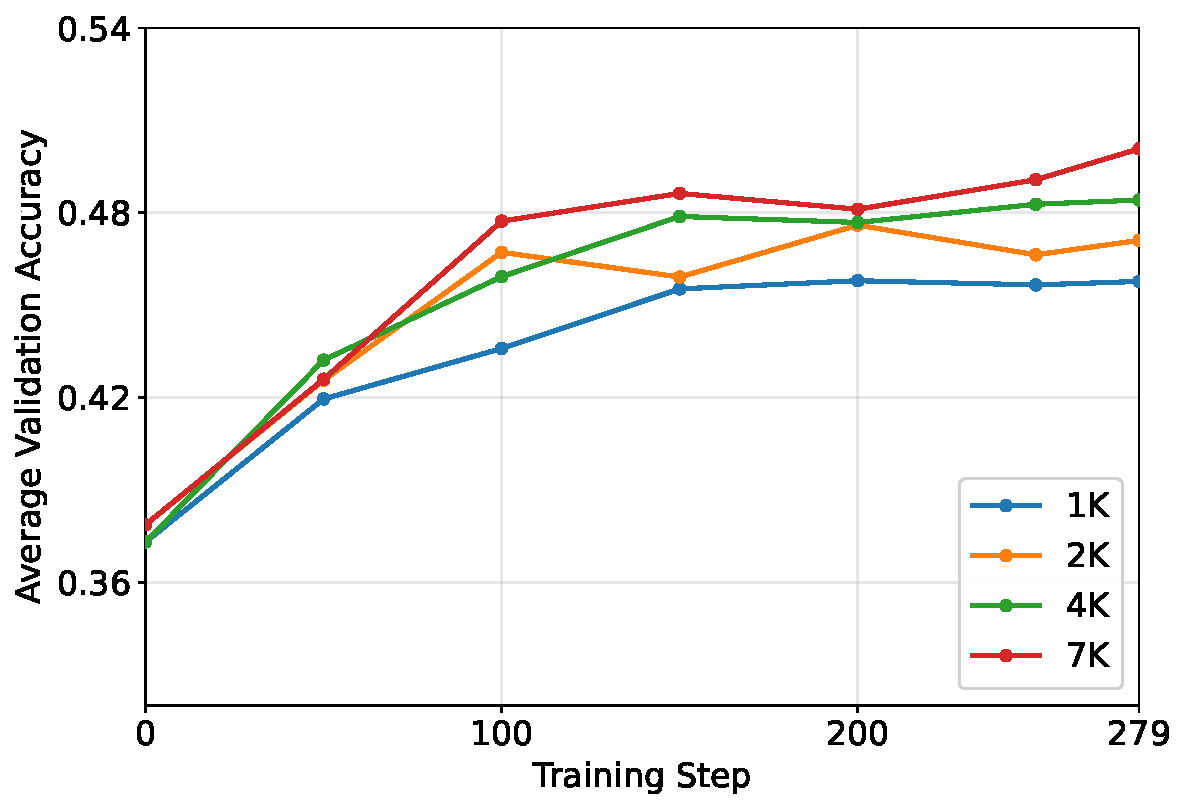
\includegraphics[width=\linewidth]{./images/length.pdf}
    \caption{\textbf{Validation performance across different maximum response length.} We compare distillation validation accuracy across training steps under $1\text{K}$, $2\text{K}$, $4\text{K}$, and $7\text{K}$ maximum token limits. }
    \label{fig:response_length_curves}
    \vspace{-1em}
\end{wrapfigure}

\textbf{Distillation Benefits from Longer CoTs} We further compare student models distilled on the hard problem $\{\pi_{954}\}$ under different maximum response length of 1024, 2048, 4096, and 7168 tokens (referred to as 1K, 2K, 4K, and 7K models, respectively). Figure \ref{fig:response_length_curves} illustrates the validation accuracy dynamics across training steps under these length limitation. The empirical results show a clear trend within the 1K to 7K token range: increasing the maximum response length enables the student model to engage in longer reasoning processes, leading to progressively higher validation accuracy. To explore the underlying mechanics, we track the token level KL loss over generation position in Figure \ref{fig:longer_cot_kl_loss}. As depicted in Figure \ref{fig:longer_cot_kl_loss}, the 7K model maintains a consistently lower KL divergence across extended generation horizons, whereas shorter variants exhibit a sharp rise in KL loss as the generation sequence lengthens. This indicates that training on longer CoT sequences directly enhances the model's longer-horizon reasoning capabilities, enabling it to sustain policy alignment with the teacher over extended context lengths.


\textbf{Harder Problems can Trigger More Reasoning Patterns.} Furthermore, we observe that training on harder problems does not simply scale token volume, but instead learns more reasoning patterns, such as self-reflection and backtracking. As shown in Figure \ref{fig:token_kl_reduction}, for the model training on easy problem ($\{\pi_{178}\}$) where trajectories are naturally short, the self-reflection token \texttt{"Alternatively"} is absent from the top-16 KL reduction list. However, it emerges in the medium model ($\{\pi_{794}\}$), and ranks higher in the hard model ($\{\pi_{954}\}$). This finding suggests that longer CoT trajectories allows the student model to acquire some sophisticated reasoning patterns that are inherently absent in shorter, simpler reasoning paths.